\documentclass{article}
\usepackage{subfig}
\usepackage{tikz}
\usepackage{siunitx}
\begin{document}
\newcommand{\imsize}{\linewidth}
\newlength\imagewidth % needed for scalebars
\newlength\imagescale % needed for scalebars
\begin{figure*}
\centering
%%%%%%%%%%%%%%%%%%%%%%%%%%%%%
	\renewcommand{\imsize}{.16\linewidth}
	\pgfmathsetlength{\imagewidth}{\imsize} % desired display width of image
	\pgfmathsetlength{\imagescale}{\imagewidth/512} % pixel width of image
	\centering
		\subfloat[Uncorrected projection images from subscans s$_1$--s$_3$, each with a size of 1024\(\times\)1024 pixels at a resolution of \SI{1.4}{\micro\meter\per pixel}, covering a FOV of approximately \SI{0.7}{\milli\meter}. The subscans s$_1$--s$_3$ overlap each other by approximately 150 pixels. 4676 projections have been acquired for the subscans s$_1$ and s$_3$, 1169 projections have been acquired for subscan s$_2$, all over a rotation of \SI{180}{\degree}.]{%
			\label{fig:s1}%
			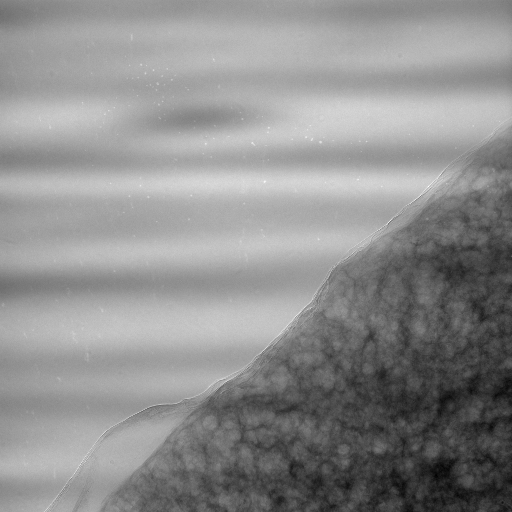
\includegraphics[width=\imsize]{R108C10B-s1}%
			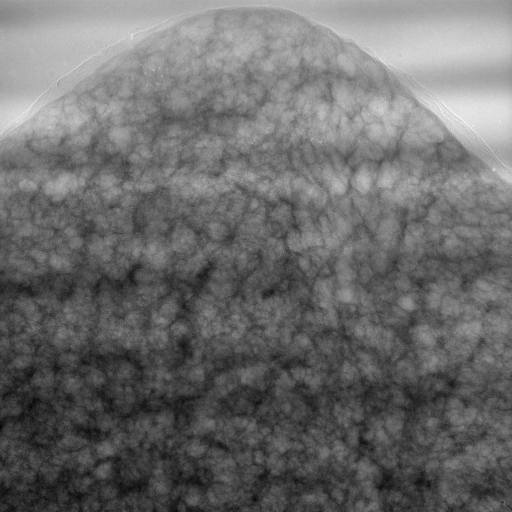
\includegraphics[width=\imsize]{R108C10B-s2}%
			\begin{tikzpicture}[x=\imagescale,y=-\imagescale]
				% place image (integer coordinates refer to pixel centers):
				\node[anchor=north west,inner sep=0pt,outer sep=0pt] at (0,0)
					{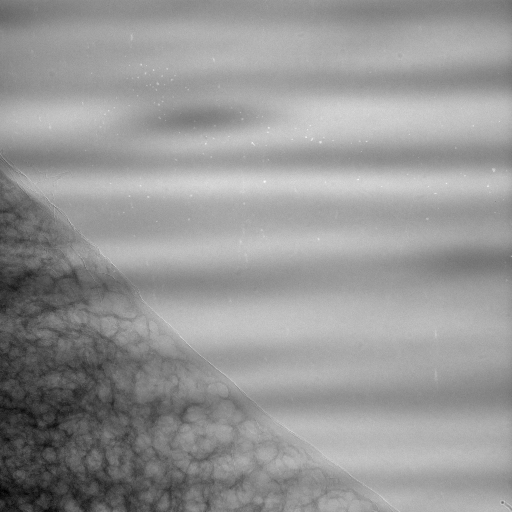
\includegraphics[width=\imagewidth]{R108C10B-s3}};
				\draw[|-|,color=white] (256-64,450) -- (512-64,450) node[midway,above] {\SI{700}{\micro\meter}};
			\end{tikzpicture}
			\label{fig:subscans}
			}
		\renewcommand{\imsize}{.48\linewidth}
		\pgfmathsetlength{\imagewidth}{\imsize} % desired displayed width of image
		\pgfmathsetlength{\imagescale}{\imagewidth/1498} % pixel width of image
		\subfloat[Merged and corrected image from the three subscans shown in subfigure~\subref{fig:subscans}. The merged projections have a size of 2994\(\times\)1024 pixels at a resolution of \SI{1.4}{\micro\meter\per pixel}. The width of the merged projections is slightly smaller than three times the width of the subscans.]{%
			\begin{tikzpicture}[x=\imagescale,y=-\imagescale]
				\node[anchor=north west,inner sep=0pt,outer sep=0pt] at (0,0)
					{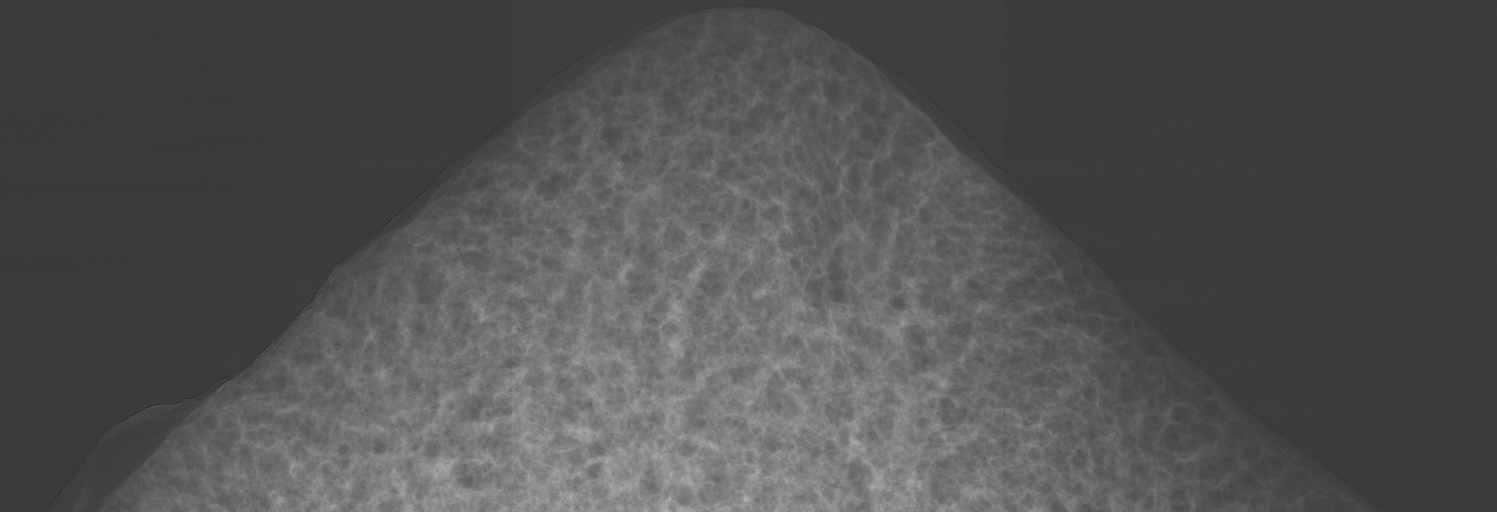
\includegraphics[width=\imagewidth]{R108C10B-merge}};
				\draw[|-|,color=white] (1242-64,450) -- (1498-64,450) node[midway,above] {\SI{700}{\micro\meter}};
			\end{tikzpicture}
			\label{fig:merge-proj}
			}
		\renewcommand{\imsize}{\linewidth}
		\pgfmathsetlength{\imagewidth}{\imsize} % desired displayed width of image
		\pgfmathsetlength{\imagescale}{\imagewidth/1365} % pixel width of image (image has been resized from 2994*1123, so that scalebar is at the same height without calculating too much...)
		\subfloat[Cropped part of one slice of the tomographic dataset reconstructed from the merged projections shown in subfigure~\subref{fig:merge-proj}. Around the sample the air-to-paraffin interface is visible due to the coherence of the x-ray beam. The bright circular shape inscribed in the square arises from the filtered back-projection, the chosen reconstruction method. The size of the cropped image is 2994\(\times\)1123 pixels. The inset shows an overview over the full slice with a size of 2994\(\times\)2994 pixels.]{%
			\begin{tikzpicture}[x=\imagescale,y=-\imagescale]
				% place image (integer coordinates refer to pixel centers):
				\node[anchor=north west,inner sep=0pt,outer sep=0pt] at (0,0)
					{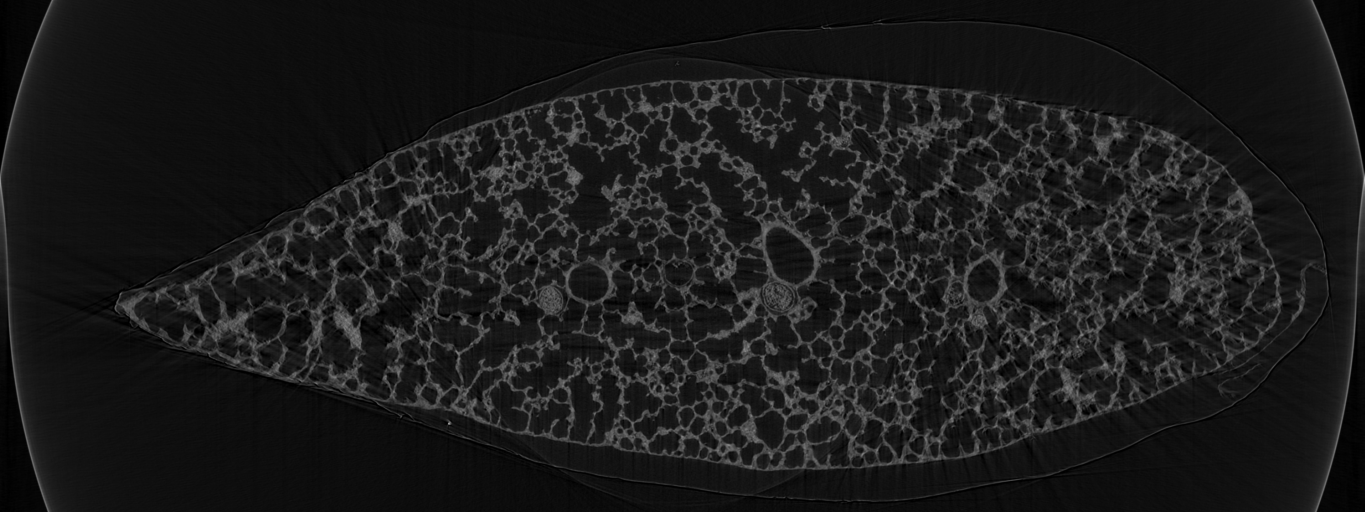
\includegraphics[width=\imagewidth]{R108C10B-merge1016-crop}};
				\newcommand{\size}{.2\imagewidth}
				\node[anchor=north west,inner sep=0pt,outer sep=0pt] at (0,0)
					{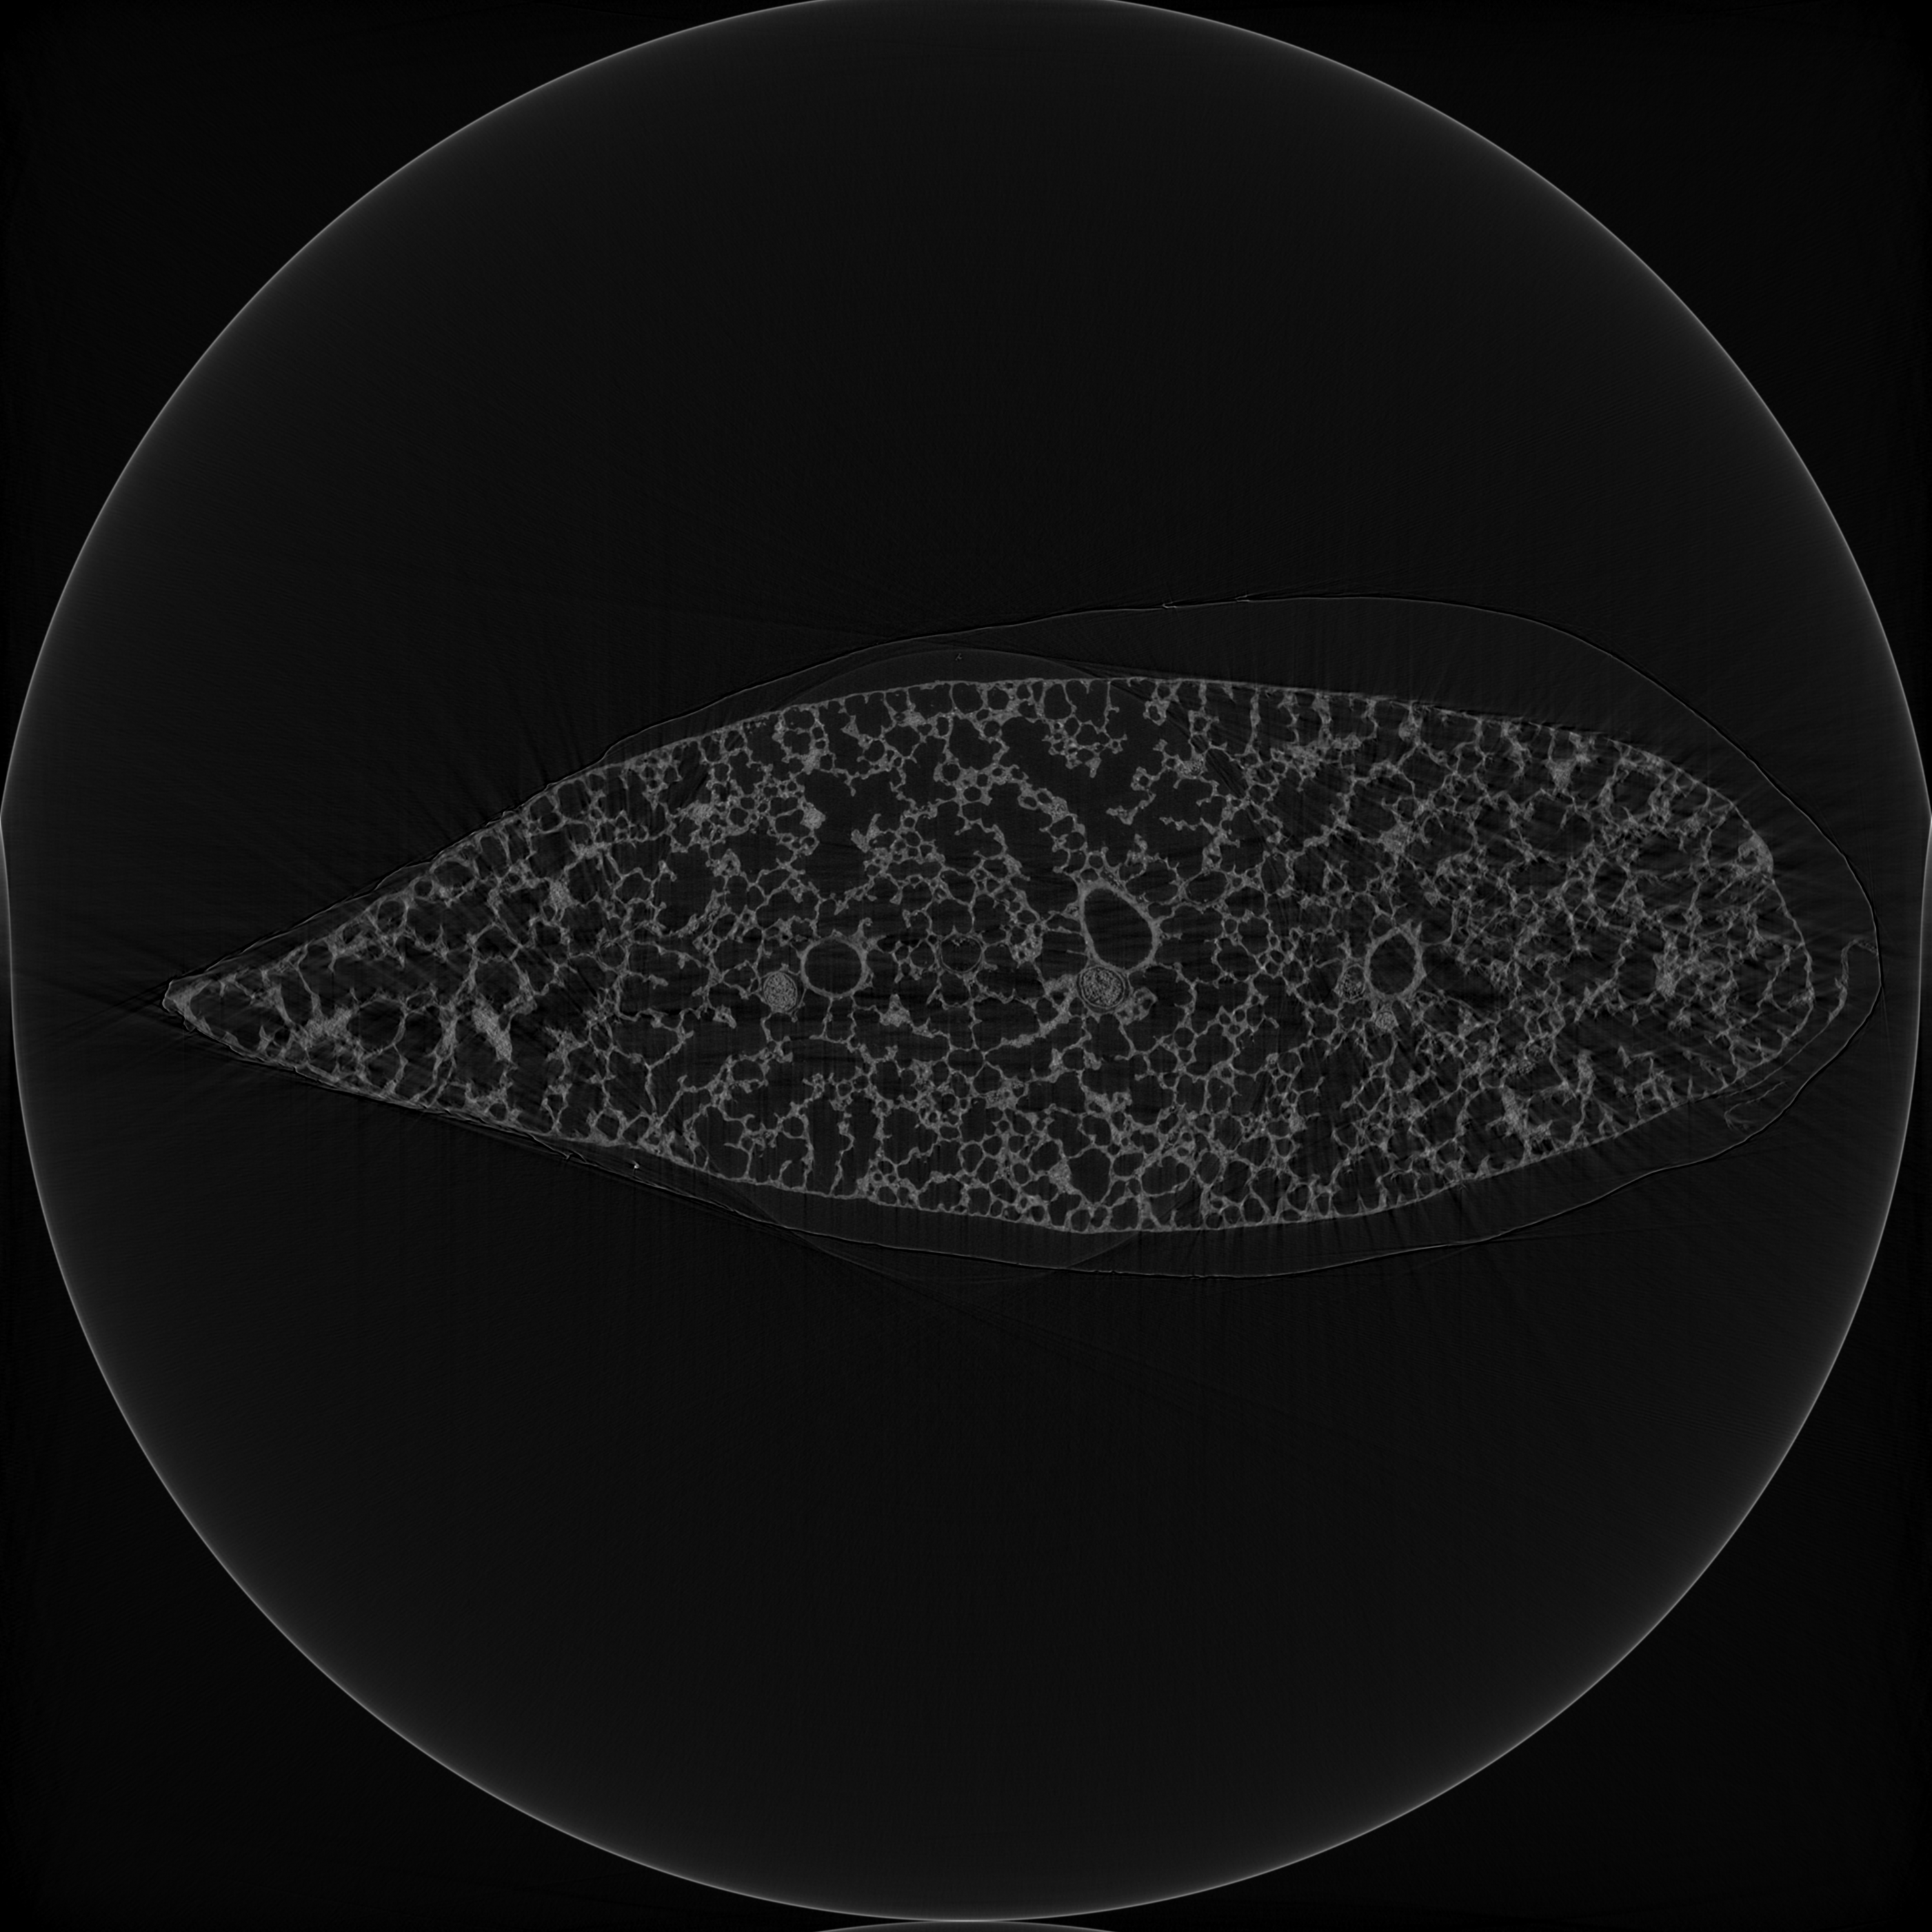
\includegraphics[width=\size]{R108C10B-merge1016}};
					\draw[white] (\size,0) -- (\size,-\size) -- (0,-\size);				\draw[|-|,color=white] (1109-64,450) -- (1365-64,450) node[midway,above] {\SI{700}{\micro\meter}};
			\end{tikzpicture}
			\label{fig:merge-rec}
			}
%%%%%%%%%%%%%%%%%%%%%%%%%%%%%	
	\caption{Different stages of a wide field scan of a rat lung sample obtained from a Sprague-Dawley rat 10 days after birth, showing the distal-medial edge of the right lower lung lobe. The sample has been scanned at \SI{12.6}{\kilo\electronvolt}.}
	\label{fig:wide field scan results}	
\end{figure*}
\end{document}